\chapter{Modeling and Forecasting of Solar Energetic Protons}
\label{chapter4}
This chapter comprises two sections. The first focuses on a modeling study concerning energetic proton acceleration and propagation from the solar corona to 1 AU. Utilizing a physics-based approach, including 3D coronal models and a 3D MAS-MHD model, we employ the EPREM model to determine fluxes and spectra of energetic protons at 1 AU, comparing results with in-situ measurements. The second part introduces a deep learning approach for forecasting the integral flux of energetic protons across three energy channels over three forecasting horizons.

\section{Introduction}
\label{sec_ch4_intro}
CMEs are pivotal in solar physics, attracting attention for their role in solar activity. Observations across various wavelengths provide insights into their dynamics \citep{vourlidas_2003, zhang_2006, bein_2011, bastian_2001, veronig_2010}. Particularly, EUV observations, aided by instruments like AIA, have become crucial in capturing early CME stages \citep{lemen_2012, pesnell_2012}. CMEs can induce shock waves in the solar corona, observable as EUV waves or CBFs, crucial for SEP acceleration \citep{thompson_1998, long_2011, ontiveross_2009, gopalswamy_2011, battarbee_2013, kozarev_2013, schwadron_2014, kong_2017}.

Previous research has focused on characterizing CME dynamics and their associated shocks, notably their relationship with CBFs \citep{kozarev_2019}. Extending this work, our study models CBF-related shock dynamics and particle acceleration up to 10\rsun, integrating with a numerical particle transport model, marking a significant advancement in Sun-to-Earth physics-based modeling \citep{kozarev_2022}.

SEP production by coronal shocks throughout the inner heliosphere has garnered attention. CMEs, particularly in their early stages, play a major role in SEP acceleration \citep{reames_1999, ontiveross_2009, gopalswamy_2011, battarbee_2013, kozarev_2013, schwadron_2014, kong_2017}. Our study extends modeling of CBF-related shock dynamics and particle acceleration, marking the first validated Sun-to-Earth physics-based modeling for SEP acceleration and transport \citep{kozarev_2022}.

Various models exist for SEP forecasting \citep{whitman_2022}, including physics-based, empirical, and Machine Learning (ML) based models. Notably, the PROSPER model provides probabilistic predictions for multiple energy channels \citep{papaioannou_2022}, while ML approaches offer promising avenues for accurate and rapid forecasting \citep{lavasa_2021, kasapis_2022}. Despite advancements, forecasting SEP fluxes remains challenging, emphasizing the need for dependable forecasting systems.
In upcoming sections, we address challenges in modeling SEP fluxes, particularly focusing on imbalanced datasets and low-resolution data. Our study builds upon previous work on CBF kinematics discussed in Chapter~\ref{chapter2} and presents advanced deep learning models for forecasting daily integral flux of SEP, offering insights into space radiation profiles.

\section{Early-Stage SEP Acceleration by CME-Driven Shocks}
\subsection{Overview}
Recent studies highlight CMEs as primary contributors to SEP production \citep{reames_1999}, especially in their early stages \citep{ontiveross_2009, gopalswamy_2011}. Advanced modeling techniques have been employed to understand CME-related shock dynamics and SEP acceleration \citep{kozarev_2019, kozarev_2016, kozarev_2022}. Our study extends this modeling up to 10\rsun, marking a significant advancement in Sun-to-Earth physics-based modeling for SEP acceleration and transport. To analyze particle fluxes at 1 AU, we utilize the SPREAdFAST framework discussed in Chapter~\ref{chapter2}.
SPREAdFAST aims to model and analyze SEP events, combining detailed CBF observations with modeling of coronal plasma and SEP production \citep{kozarev_2022}. Its components include CBF kinematics modeling, coronal shock and particle acceleration modeling, interplanetary particle transport modeling, and comparison with observations from instruments like SOHO and ERNE. This comprehensive framework enhances our understanding and forecasting capabilities for SEP events, contributing to advancements in Sun-to-Earth physics-based modeling.

\subsection{Coronal SEP Acceleration}
Utilizing the coronal Diffusive Shock Acceleration (DSA) model \citep{kozarev_2016, kozarev_2019}, we calculate proton acceleration dynamics from the low corona to 10\rsun, employing remote solar observations and data-driven model output from the CASHeW framework. The model incorporates shock parameters along multiple shock-crossing field lines to compute proton injection momenta and subsequent distribution function spectra or fluxes. Its validity is confirmed through analysis of several SEP events.

\subsection{Input Data and Spectral Fitting}
We utilize suprathermal proton spectra obtained from 1 AU fluxes recorded by the SOHO/ERNE instrument \citep{torsti_1995} as input data, fitted with power laws in the energy range of 0.056–3.0 MeV. These spectra serve as input for the DSA model, allowing detailed examination of proton acceleration dynamics under CME-driven shocks.

\subsection{Transport of SEPs and Comparison with ERNE Observations}
To model the transport of accelerated SEPs to 1 AU, we employ a modified version of the Energetic Particle Radiation Environment Module \citep[EPREM]{schwadron_2010}. This model incorporates essential effects such as pitch-angle scattering, adiabatic focusing and cooling, convection, streaming, and stochastic acceleration. Comparison with ERNE observations is conducted, assessing the agreement between modeled and observed proton fluences and onset times.
The methodology involves selecting events meeting specific criteria, characterizing CBF kinematics using the CASHeW framework, and comparing modeled and observed proton fluences through scatter plots and Mean Squared Logarithmic Error (MSLE).

\subsection{Results and Discussions}
Modeling the dynamics of shock waves and particle acceleration in the solar corona yields insights into solar particle radiation. The study underscores the coronal environment's pivotal role in SEP acceleration and transport. It reveals that coronal structures and particle energy significantly influence SEP production during CME-driven shocks. Continuous changes in acceleration occur due to plasma parameter gradients. This understanding aids in spatial distribution and energy dependence assessment of SEPs. Moreover, the SPREAdFAST framework shows promise for SEP event forecasting and space weather prediction. Discrepancies between modeled and observed fluxes, particularly at higher energies, suggest the need for refining the modeling framework to better align with observations.

%%%%%%%%%%%%%%%%%%%%%%%%%%%%%%%%%%%%%%%%%%%%%%%%%%%%%%%%%%%%%%%%%%%%%%%%%%%%%%%%%

\section{Solar Proton Flux Forecasting with Deep Learning Models}
\subsection{Data Preparation}
This section outlines the selection of input physical quantities, their sources, and the forecasting outputs. Two categories of input features are considered: remote signatures and in-situ measurements. Remote signatures include the F10.7 index, long-wavelength ($X_L$), and short-wavelength ($X_S$) x-ray fluxes, obtained from the GOES database\footnote{GOES SXR Database: \url{https://satdat.ngdc.noaa.gov/sem/goes/data/avg/}}. In-situ measurements comprise near-Earth solar wind magnetic field and plasma parameters, sourced from spacecraft stationed at the Lagrange point (L1)\footnote{OMNI Database: \url{https://omniweb.gsfc.nasa.gov}}. Data covering December 1976 to July 2019 were acquired from the Space Physics Data Facility (SPDF) OMNIWeb database and supplemented with daily sunspot numbers from the SILSO archive\footnote{Sunspot Number Dataset: \url{https://www.sidc.be/silso/home}}.

Figure~\ref{fig_allFeatures} displays the timeseries data for all features, including SEP integral fluxes, sunspot numbers, F10.7 index, x-ray fluxes, solar wind speed, and IMF magnitude. The dataset was split into training, validation, and test sets for deep learning model development \citep{ripley_2007}. Correlation analysis guided the selection of input parameters, focusing on logarithms of SEP fluxes, x-ray fluxes, F10.7 index, sunspot numbers, solar wind speed, and IMF magnitude. Separate models were trained for each target output feature.
To ensure consistency, all timeseries data durations were aligned and resampled to daily averages. Missing values were linearly interpolated. The dataset split followed a 9-2-1 strategy over the 43-year timeframe, allocating 74.29\% to training, 16.2\% to validation, and 9.51\% to testing. This strategy aimed to mitigate bias and streamline training efficiency, without shuffling timeseries data to maintain temporal order \citep{mnedal_2019, pala_2019, benson_2020, zhang_lstm_2022, zhu_2022}.

\begin{figure}[!htp]
	\centering
	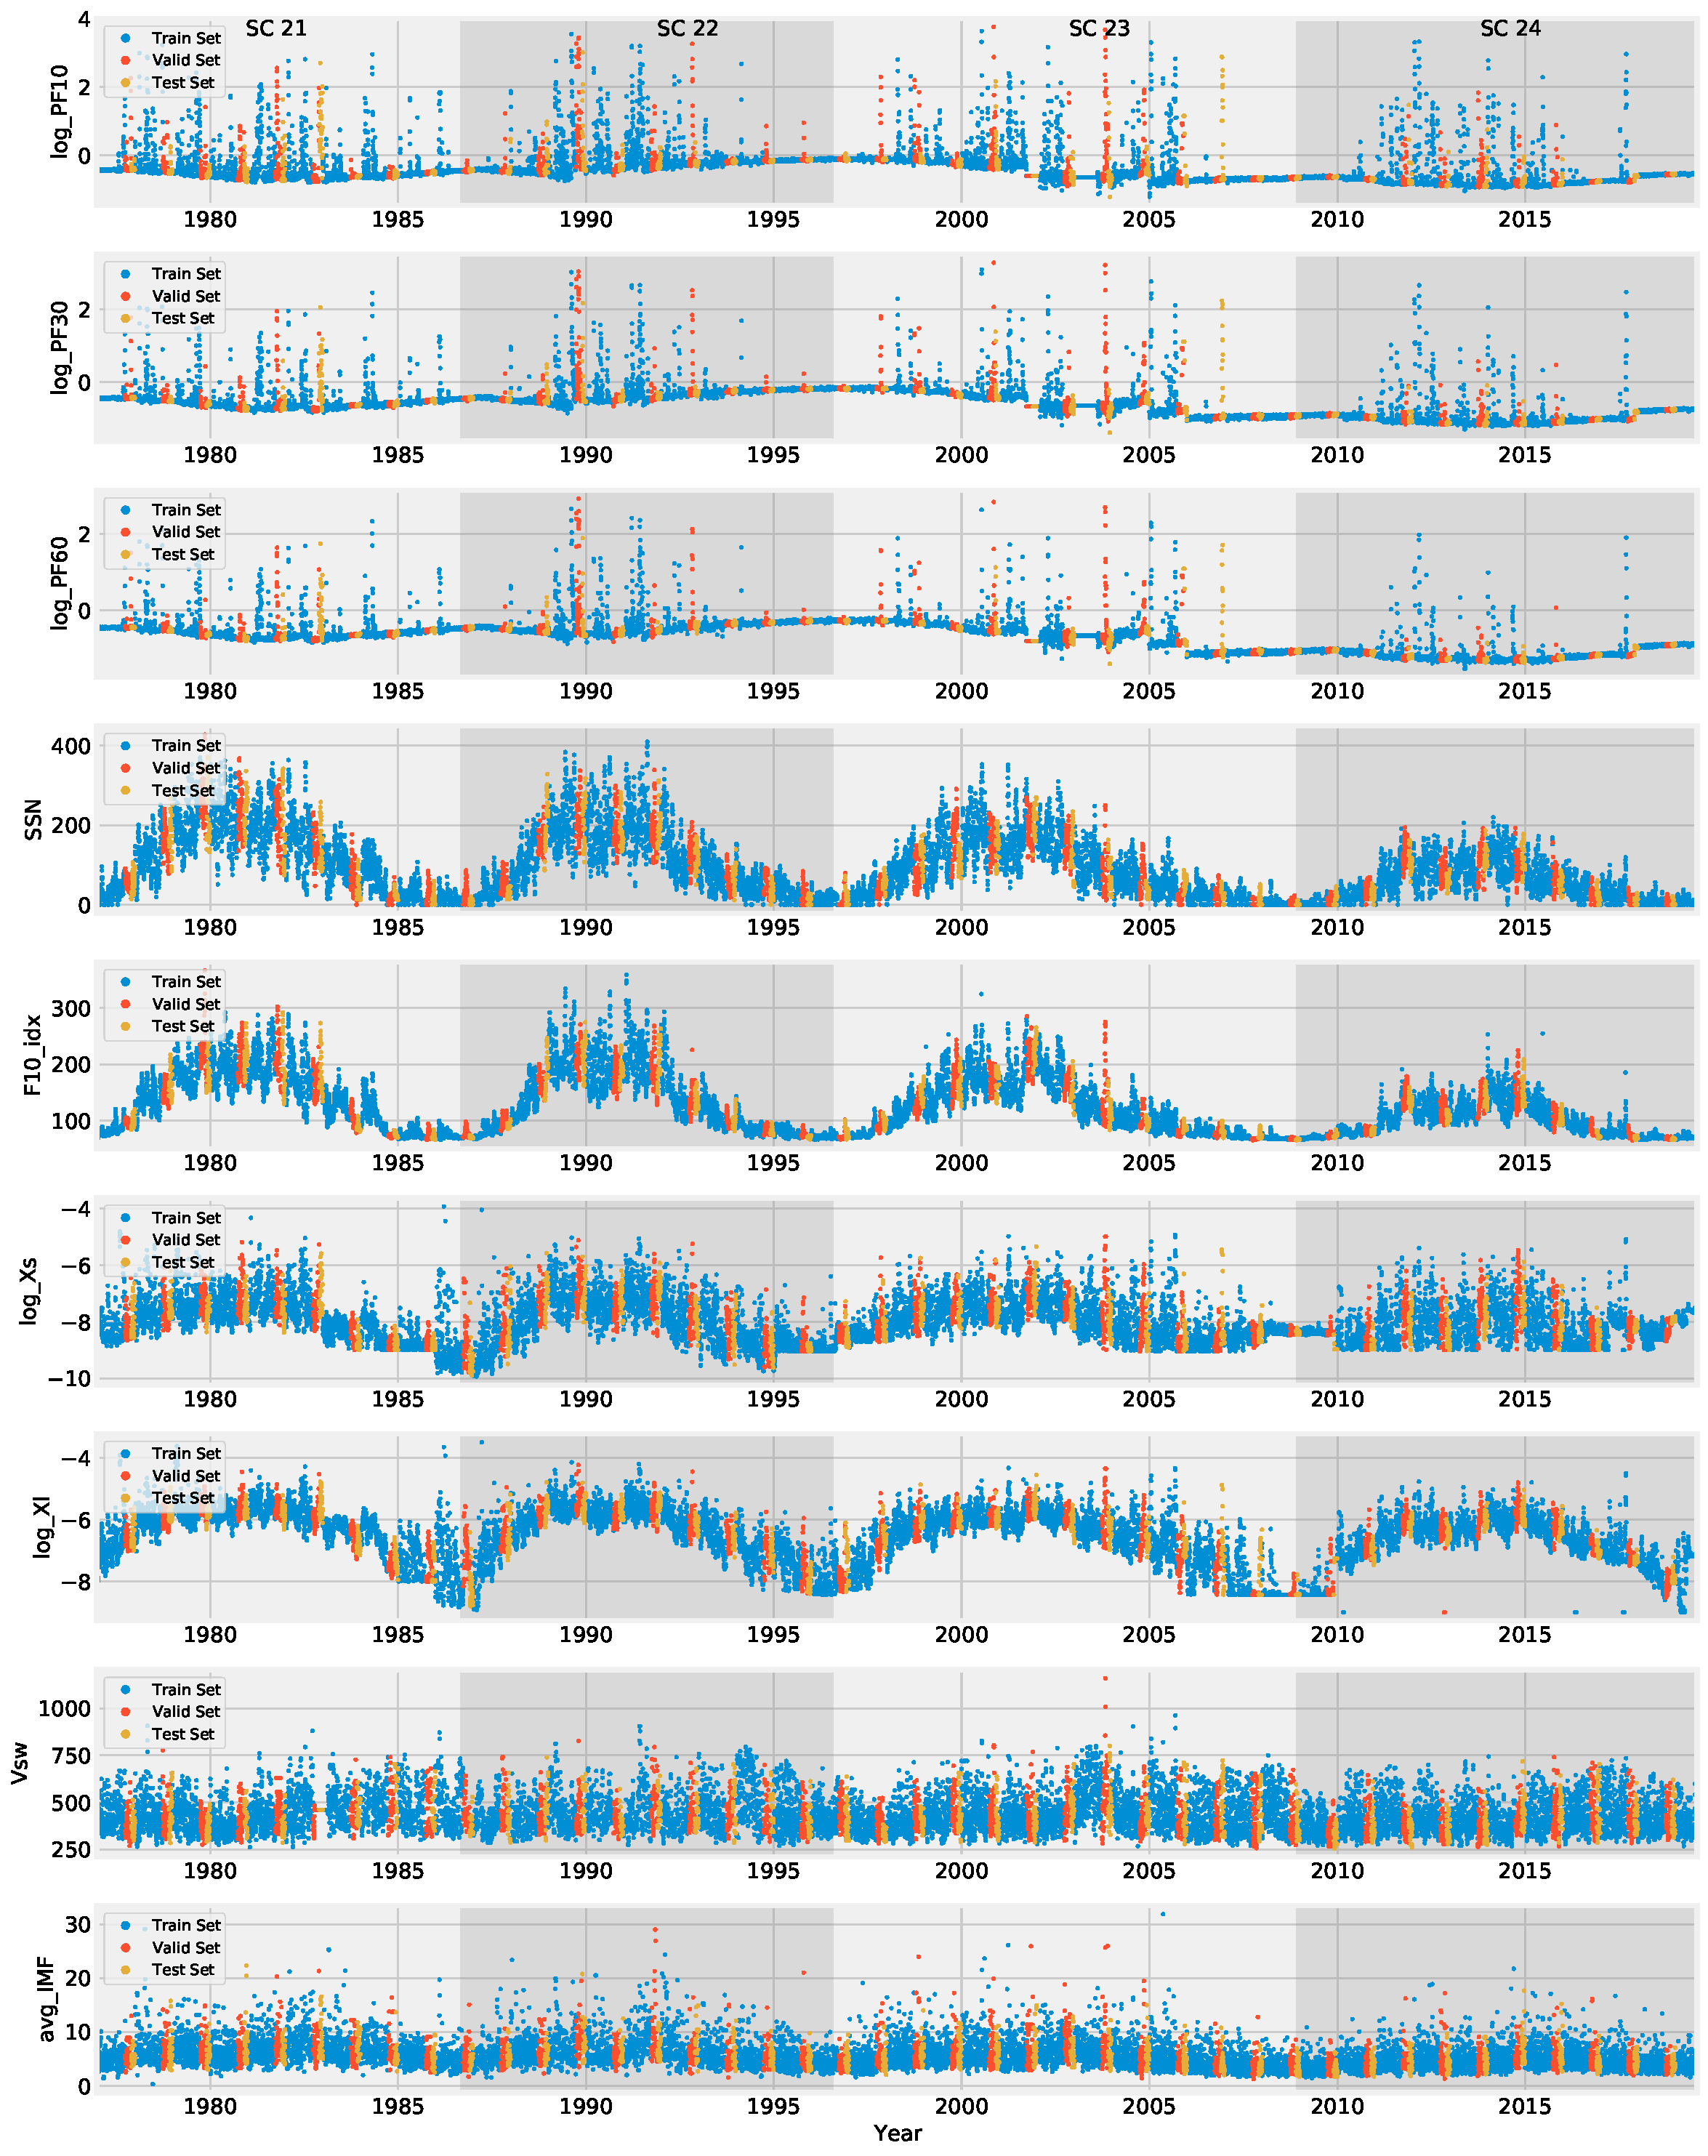
\includegraphics[width=0.9\textwidth]{chapter4/figs/subplots_dataSplit_allFeatures.pdf}
	\caption{Data splitting for all input features, showing the training, validation, and testing sets. Daily data from 1976-12-25 00:00 to 2019-07-30 00:00. The gray shading labels the solar cycles from SC21 to SC24.}
	\label{fig_allFeatures}
\end{figure}

\subsection{Method}
This section outlines the data analysis methods employed in this study. It begins with an overview of model selection, followed by a detailed explanation of the Bi-directional Long Short-Term Memory (BiLSTM) neural network architecture.

\subsubsection{The Bi-LSTM Model}
BiLSTM neural networks, an extension of recurrent neural networks (RNNs), process input sequences in both forward and backward directions \citep{schuster_1997, hochreiter_1997, kolen_2001}. Unlike regular RNNs, which rely solely on past information, BiLSTM networks incorporate future context, enhancing prediction accuracy. Each BiLSTM layer comprises forward and backward LSTM layers, as depicted in Figure~\ref{fig_model}, enabling the model to capture long-term dependencies effectively.

BiLSTM networks offer several advantages over traditional LSTM networks \citep{graves_2005, ihianle_2020, alharbi_2021}. They excel in tasks like timeseries forecasting, speech recognition, and language translation by capturing long-term dependencies in both directions \citep{wollmer_2013, graves_2014, sundermeyer_2014, huang_2018, nammous_2022}. Additionally, they adapt well to variable-length sequences and handle noisy data. However, BiLSTM networks are computationally intensive, require more parameters, and demand larger training datasets.

The final dataset comprises 7 features, spanning from December 25$^{th}$, 1976, to July 30$^{th}$, 2019, totaling 15,558 samples. The model configuration includes 4 BiLSTM layers with 64 neurons each and an output dense layer with 3 neurons representing the forecasting horizon. The total number of trainable parameters is 333,699. Training involved 50 epochs, as further iterations did not yield significant improvements.
Callbacks such as \textit{ModelCheckpoint}, \textit{EarlyStopping}, and \textit{ReduceLROnPlateau} were employed to monitor model performance, minimize overfitting, and adjust learning rate, respectively.

\begin{figure}[!htp]
	\centering
	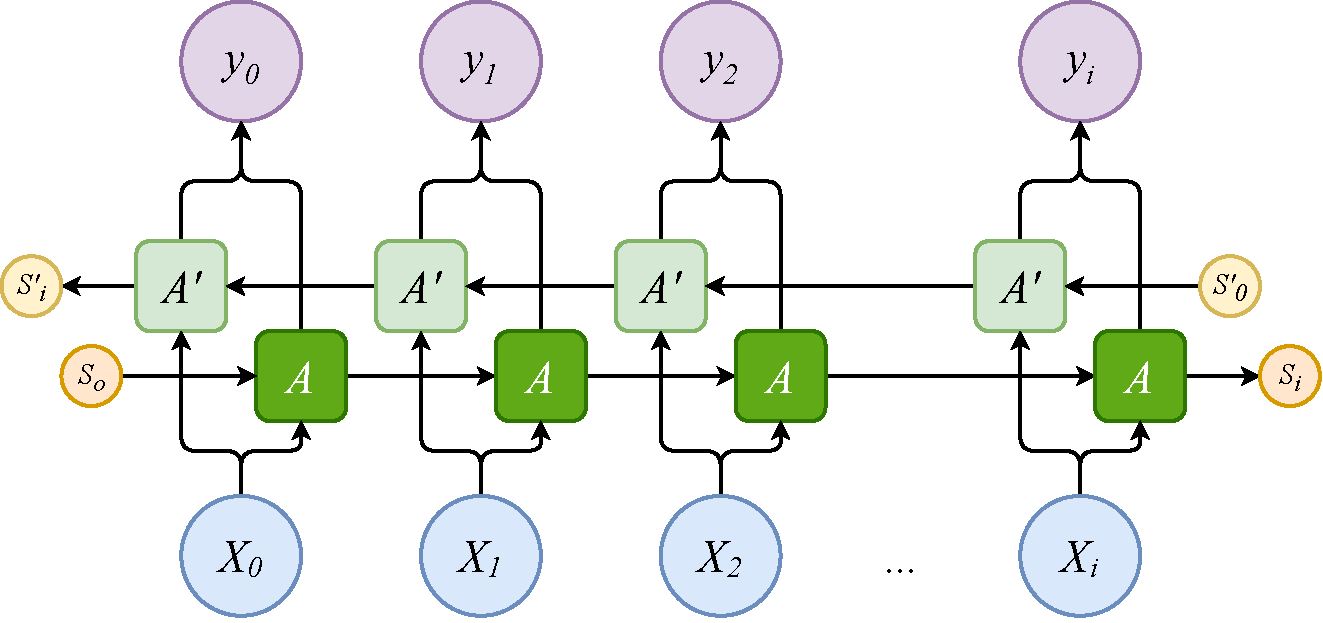
\includegraphics[width=0.6\textwidth]{chapter4/figs/diagram.drawio.pdf}
	\caption{Architecture of a single BiLSTM layer. The blue circles at the bottom labeled by \textit{($x_0$, $x_1$, $x_2$, ..., $x_i$)} are the input data values at multiple time steps. The purple circles, on the other hand, are the output data values at multiple time steps labeled by \textit{($y_0$, $y_1$, $y_2$, ..., $y_i$)}. The dark green and light green boxes are the activation units of the forward and backward layers, respectively. The orange and yellow circles are the hidden states at the forward and backward layers, respectively. Both the forward and backward layers composes a single hidden BiLSTM layer. The figure is adopted from \citet{olah_2015}}
	\label{fig_model}
\end{figure}

\subsubsection{Model Selection}
To determine the most suitable model, I conducted a comprehensive analysis, starting with baseline models like the naive (persistence) model and moving-average model. Following this, I explored ML-based models, opting for the Adaptive moment estimation (Adam) optimizer for its efficiency \citep{kingma_2015}.

Data preparation involved creating a windowed dataset using a Multi-Input Multiple Output (MIMO) strategy, minimizing the imbalance of active and quiet days \citep{benson_2020}. The Huber loss function was selected due to its robustness to outliers, crucial for our noisy data.

Various neural network architectures were examined, including linear models, dense ML models, simple RNNs, LSTM, and BiLSTM models. Optimal learning rates were determined using the LearningRateScheduler callback function. Ultimately, a BiLSTM model with five hidden layers, each comprising 64 neurons, and a learning rate of 0.001 was chosen based on performance evaluation on validation and test sets.
Figure~\ref{fig_benchmark} illustrates the comparative analysis of Huber loss across the evaluated models. Multiple evaluation metrics were utilized to assess model accuracy and performance, guiding further refinement.

\begin{figure}[!htp]
	\centering
	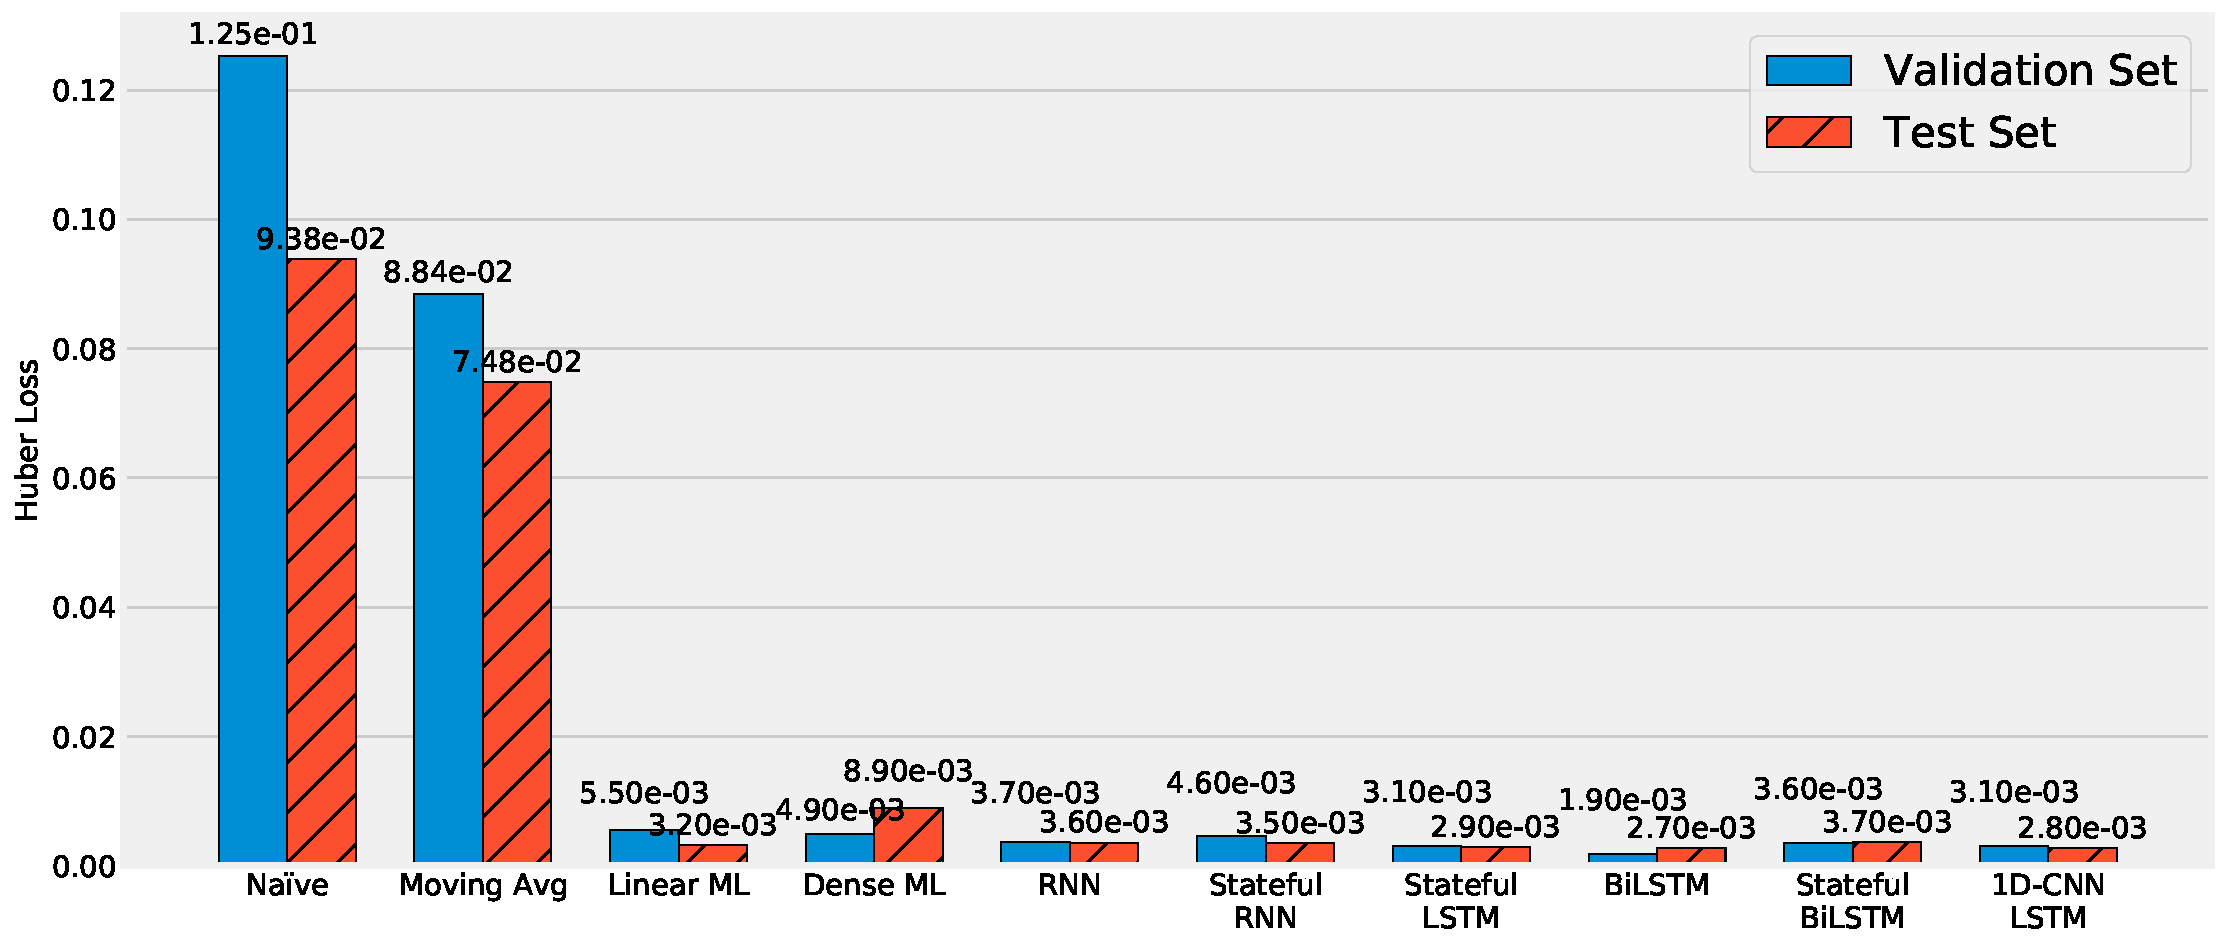
\includegraphics[width=\textwidth]{chapter4/figs/models_benchmark.pdf}
	\caption{Benchmarking of 10 models, shows the Huber loss for the validation and test sets.}
	\label{fig_benchmark}
\end{figure}

\subsection{Results and discussion}
\subsubsection{Long-term Forecasting}
In Figure~\ref{fig_benchmark}, ML-based methods showed similar performance, outperforming persistence and moving average models. The BiLSTM model exhibited superior performance across validation and test sets.

Three BiLSTM models, one per energy channel, were developed and trained to forecast SEP integral flux. Model performance was evaluated using Huber loss (Fig.~\ref{fig_lossCurve}), MAE, and learning rate adjustments via \textit{LearningRateScheduler} callback function.

Experimentation revealed batch size and optimizer learning rate as critical hyperparameters affecting model performance \citep{greff_2016}. Other architectural changes yielded marginal improvements but increased training time and computational resources.

Figure~\ref{fig_model_vs_obs_tstset} depicts model predictions against observations for 1-day, 2-day, and 3-day forecasts across energy channels. Correlation analysis on the out-of-sample test set showed high correlation across forecast windows.
Correlation between modeled data and observations declined with longer forecast horizons, especially noticeable between 1 and 1.5 on the x-axis. Rolling window analysis (Fig.~\ref{fig_crosscorr_tstset}) revealed correlation drops during solar cycle transitions.

During low solar activity, forecasting low SEP fluxes becomes challenging due to increased randomness. Factors influencing correlation during quiet periods require further investigation.

Model performance ranked highest for $>$60 MeV, followed by $>$10 MeV and $>$30 MeV channels. Correlation decline at $>$30 MeV is consistent with previous findings \citep{le_2017}.

Visual inspection of test set examples (Fig.~\ref{fig_model_vs_obs_tstset}) revealed strong correlation between predicted and observed onset time, peak time, and end times of SEP events. This suggests that the model effectively captures temporal variations and flux trends in SEP events.

Evaluation using skill scores and threshold-based clustering algorithm demonstrated declining performance with longer forecasting windows. Our model showed comparable performance with previous studies (Table~\ref{table_skillscores_comparison}), with lower false alarm rate compared to UMASEP model.

\begin{figure}[!htp]
	\centering
	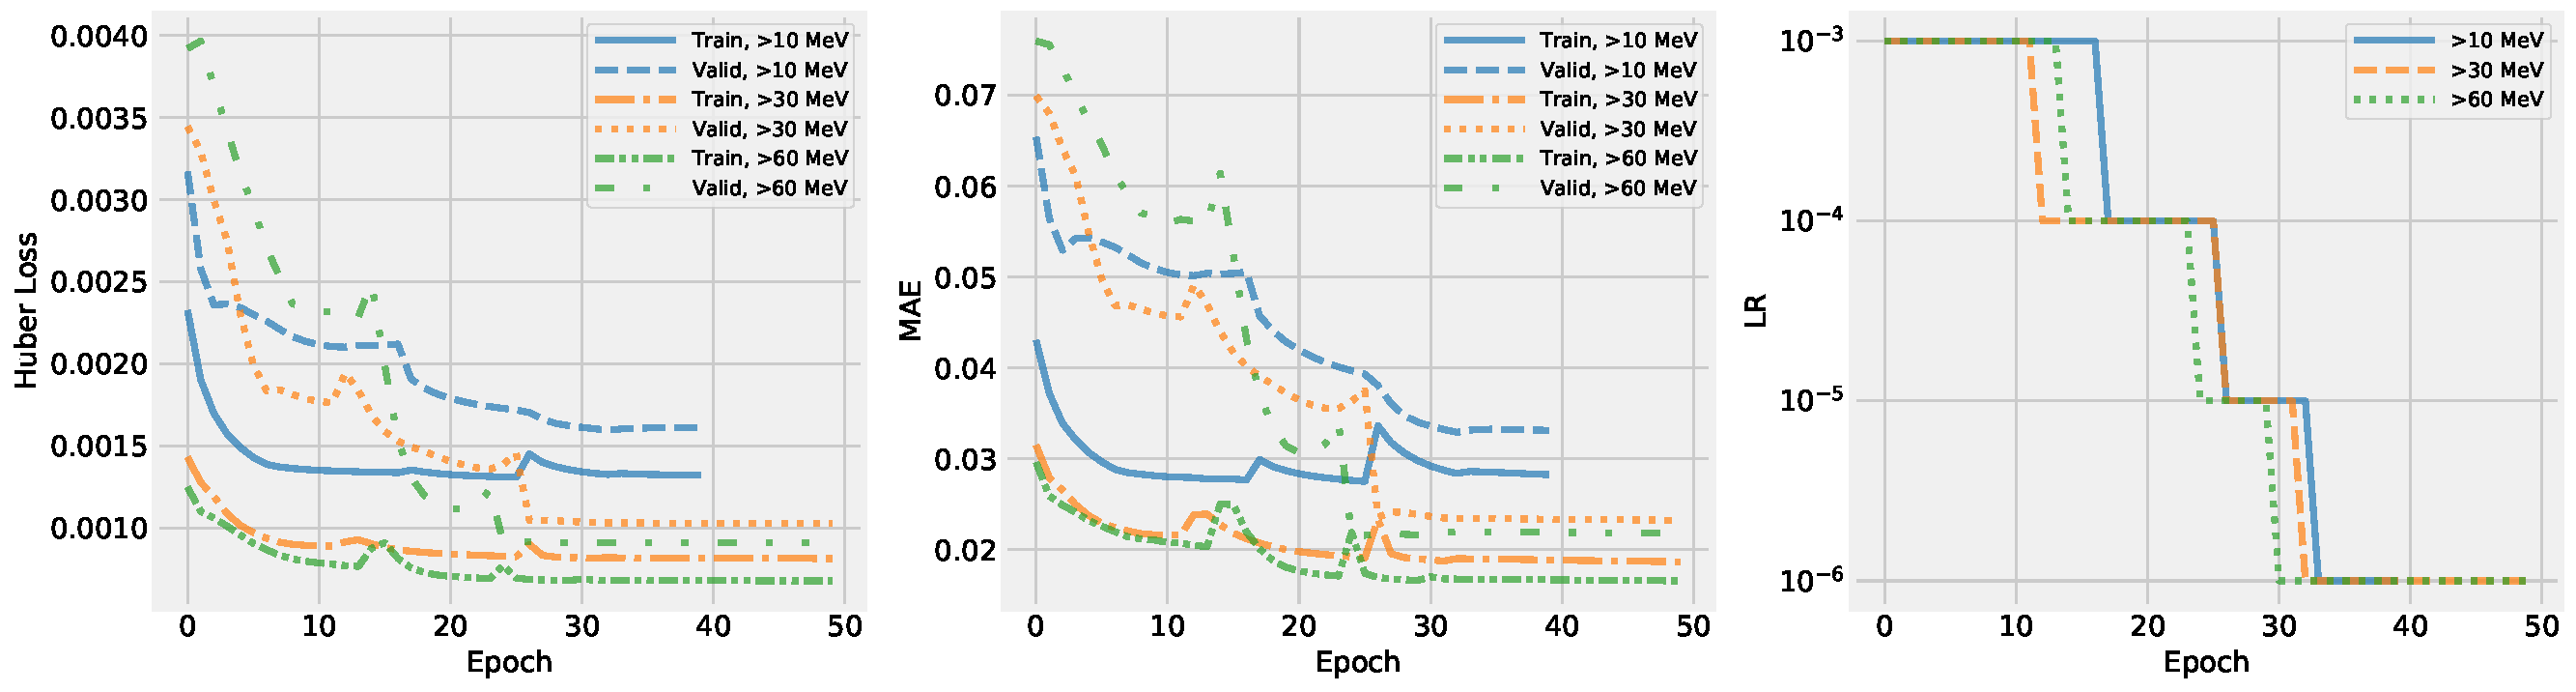
\includegraphics[width=\textwidth]{chapter4/figs/loss_curve_allenergies.pdf}
	\caption{\textit{Left Panel} - The Huber loss vs. the number of training epochs for the BiLSTM model for the validation and test sets, for the 3 energy channels. \textit{Middle Panel} - The mean absolute error (MAE); the model's metric vs. the number of training epochs. \textit{Right Panel} - Shows how the learning rate of the Adam optimizer changes over the number of epochs.}
	\label{fig_lossCurve}
\end{figure}

\begin{figure}[!htp]
    \centering
    \begin{subfigure}{0.4\textwidth}
         \centering
         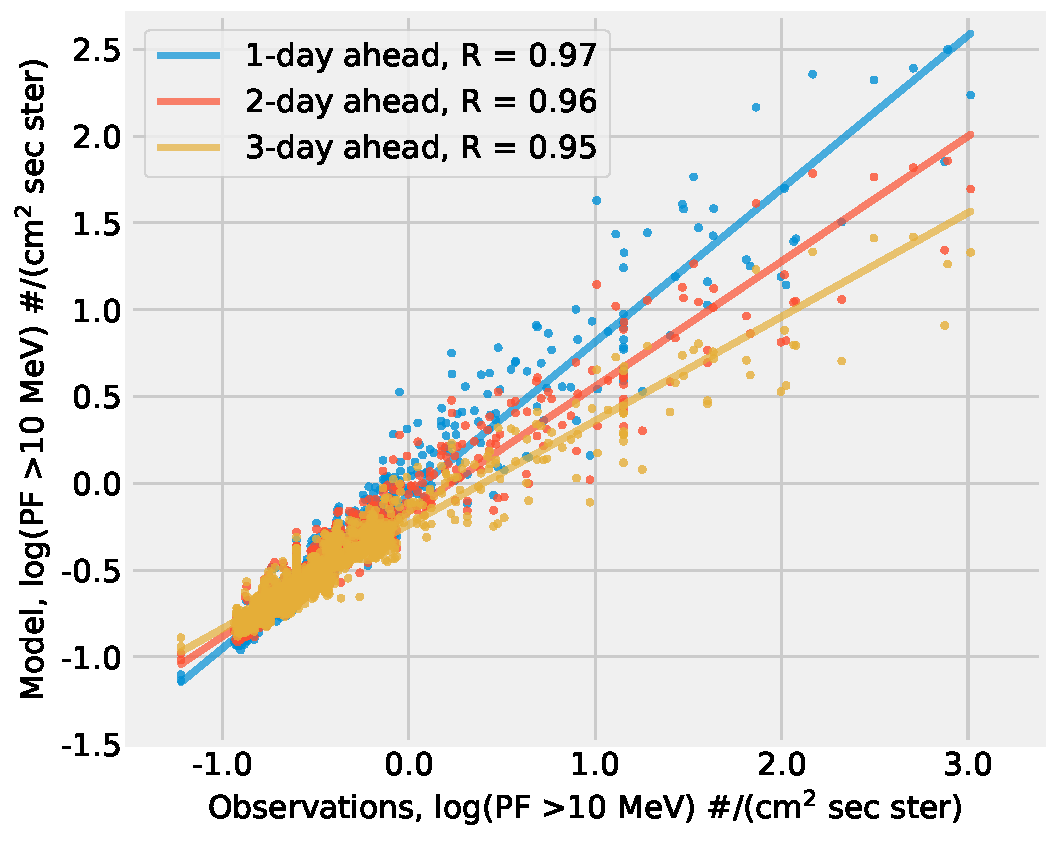
\includegraphics[width=\textwidth]{chapter4/figs/scatterplot_obs_vs_model_tstset_3in1_log_PF10.pdf}
    \end{subfigure}
    %\hfill
    \begin{subfigure}{0.4\textwidth}
         \centering
         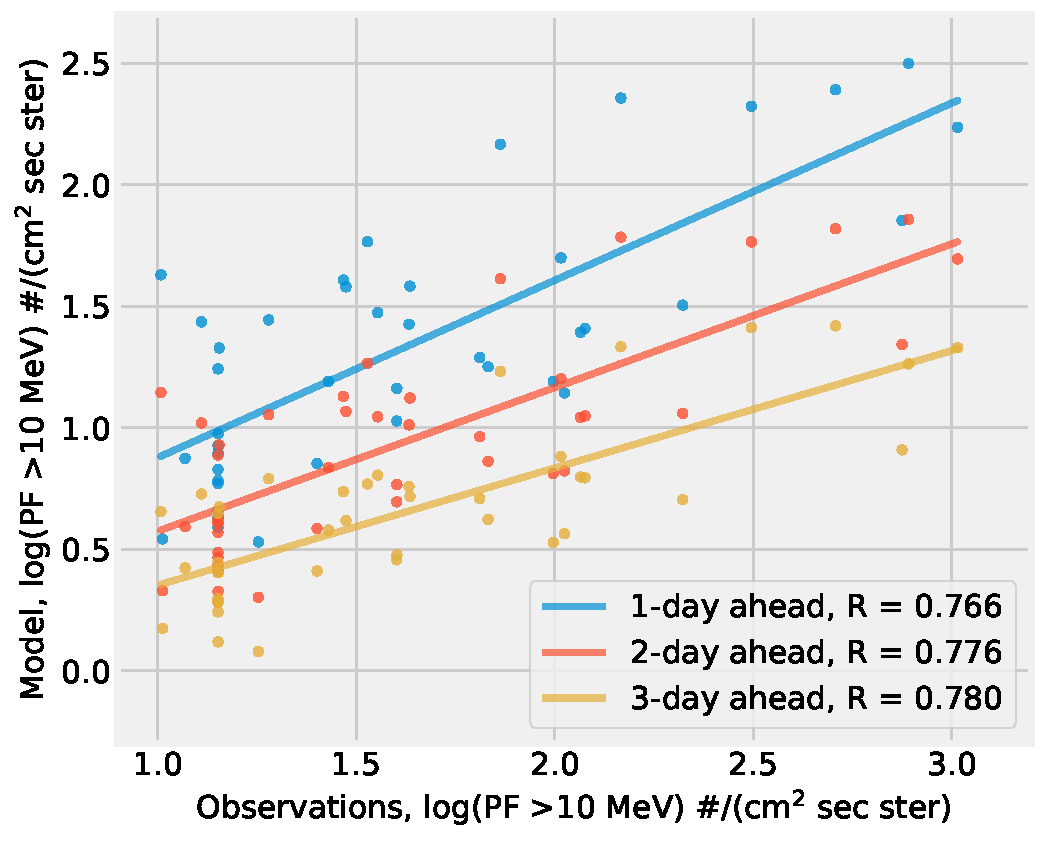
\includegraphics[width=\textwidth]{chapter4/figs/scatterplot_obs_vs_model_tstset_3in1_LOG_PF_LT1_log_PF10.pdf}
    \end{subfigure}
    \begin{subfigure}{0.4\textwidth}
         \centering
         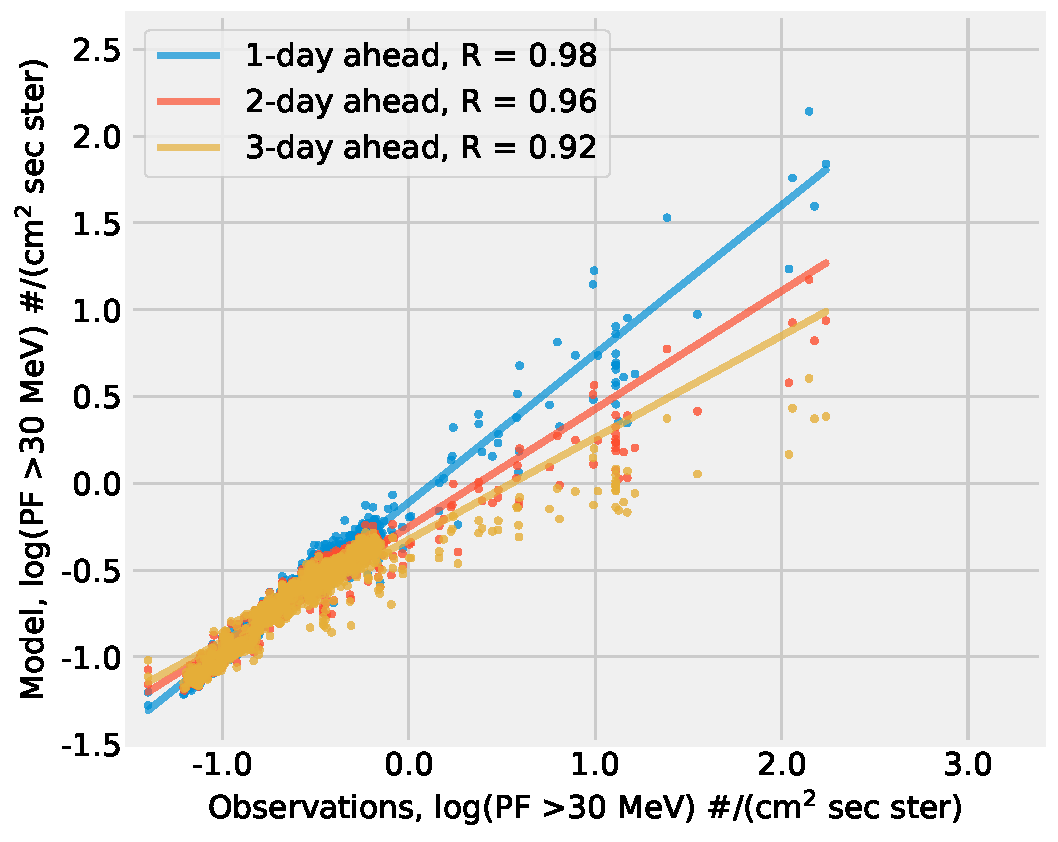
\includegraphics[width=\textwidth]{chapter4/figs/scatterplot_obs_vs_model_tstset_3in1_log_PF30.pdf}
    \end{subfigure}
    %\hfill
    \begin{subfigure}{0.4\textwidth}
         \centering
         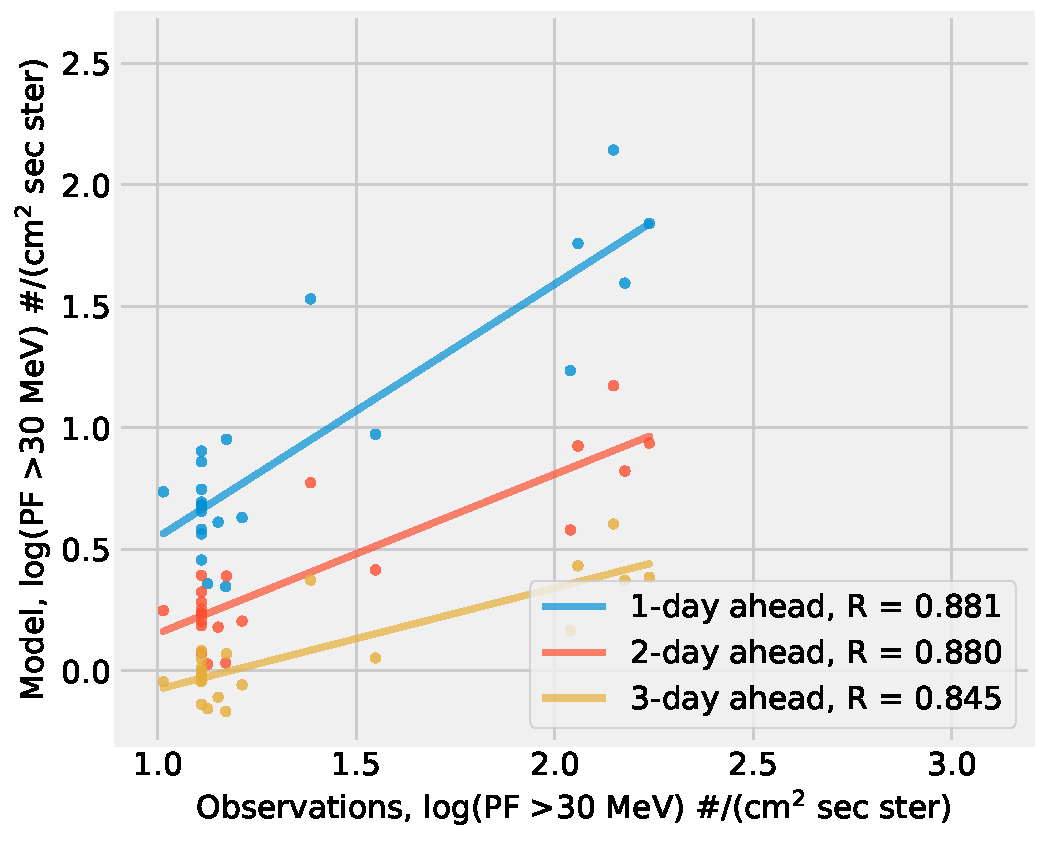
\includegraphics[width=\textwidth]{chapter4/figs/scatterplot_obs_vs_model_tstset_3in1_LOG_PF_LT1_log_PF30.pdf}
    \end{subfigure}
    \begin{subfigure}{0.4\textwidth}
         \centering
         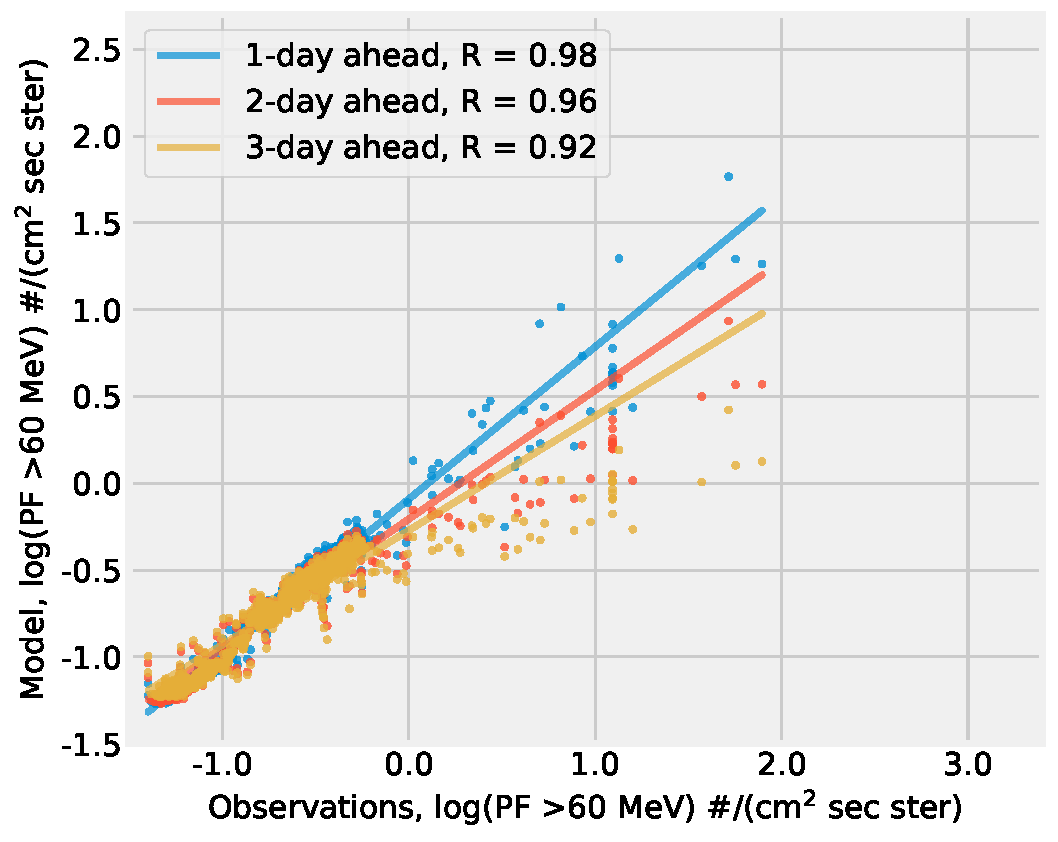
\includegraphics[width=\textwidth]{chapter4/figs/scatterplot_obs_vs_model_tstset_3in1_log_PF60.pdf}
    \end{subfigure}
    %\hfill
    \begin{subfigure}{0.4\textwidth}
         \centering
         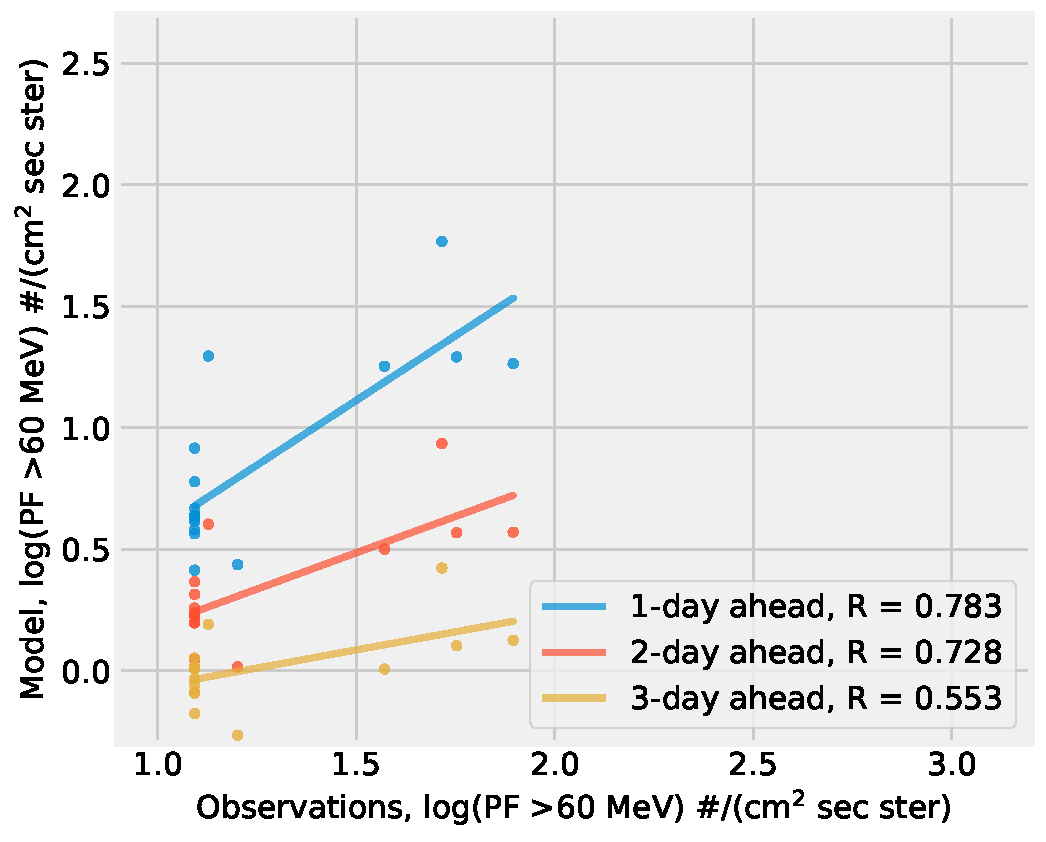
\includegraphics[width=\textwidth]{chapter4/figs/scatterplot_obs_vs_model_tstset_3in1_LOG_PF_LT1_log_PF60.pdf}
    \end{subfigure}
	\caption{Correlation between the model predictions and observations for 1-day, 2-day, and 3-day ahead for $>$10 MeV (top panel), $>$30 MeV (middle panel), and $>$60 MeV (bottom panel). The panels in the left column represent all the points of the test set, those in the right column represent all the observations points with daily mean flux $\geq$10 pfu.}
	\label{fig_model_vs_obs_tstset}
\end{figure}

\begin{figure}[!htp]
	\centering
    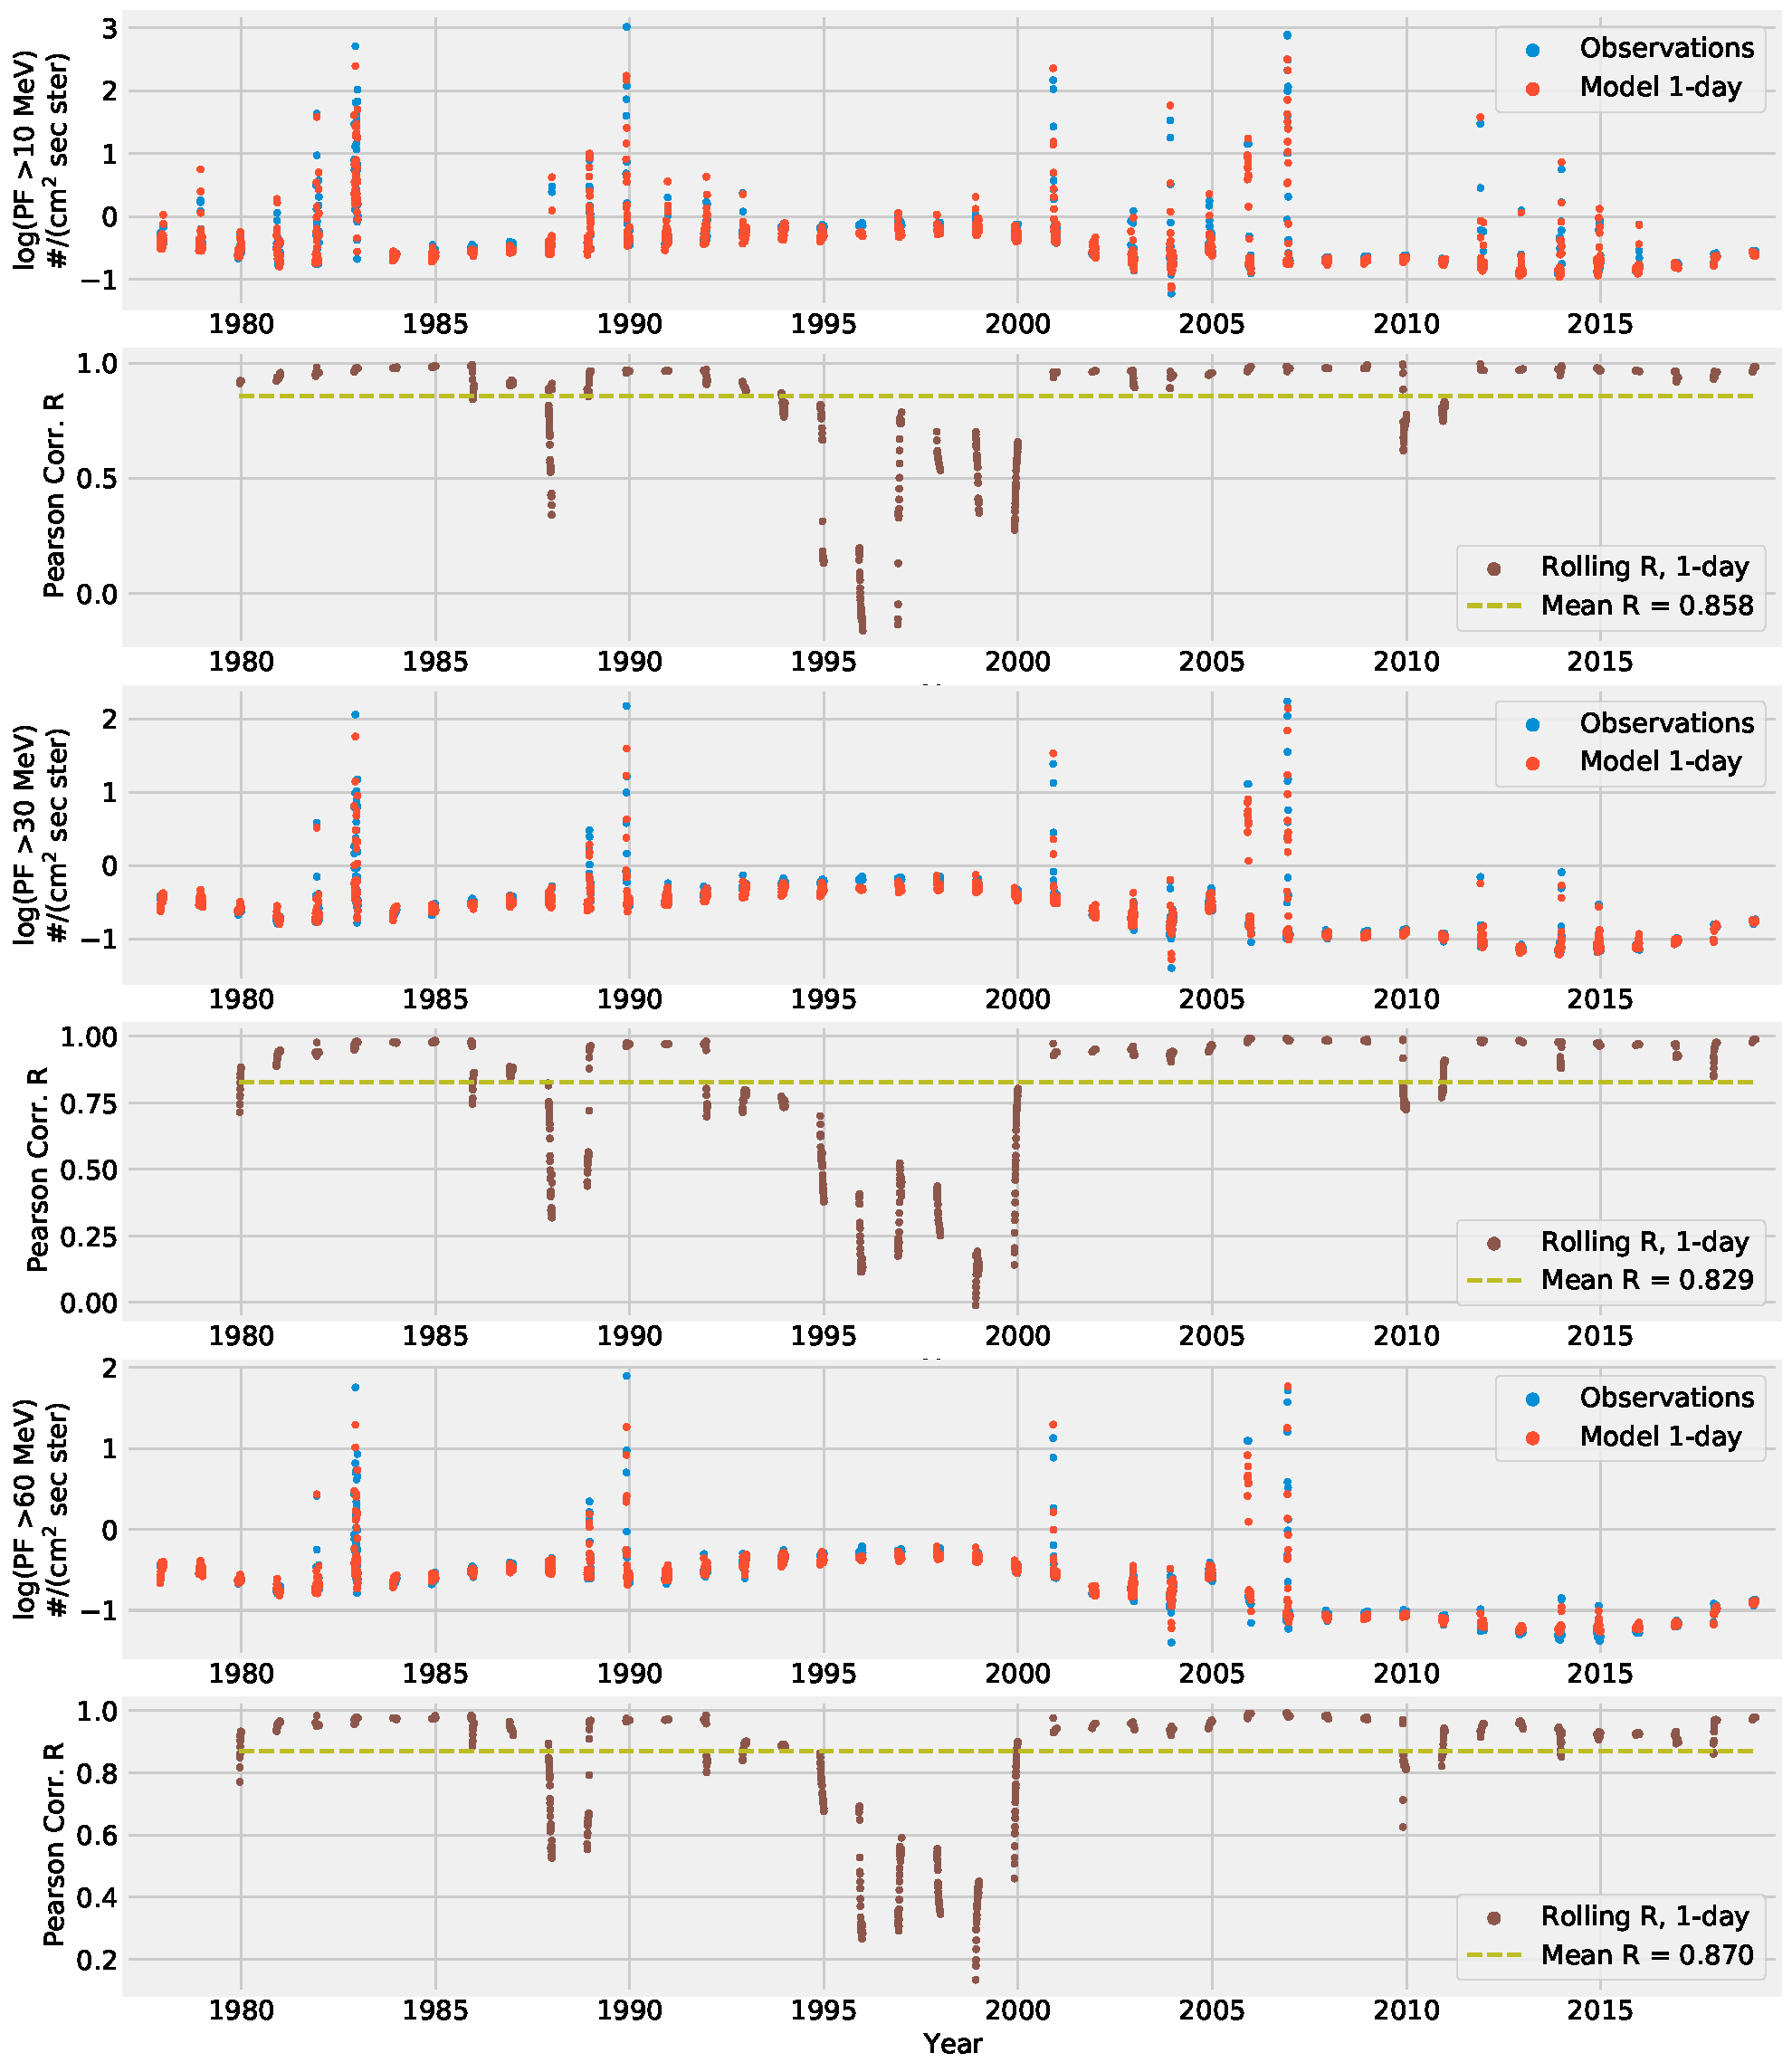
\includegraphics[width=\textwidth]{chapter4/figs/comparison_crosscorr_tstset_1day_3channels.pdf}
    \caption{Comparison between the model outputs and observations of the test set for the 3 energy channels. In addition to the rolling-mean window correlation for 1-day ahead predictions.}
\label{fig_crosscorr_tstset}
\end{figure}

\begin{figure}[!htp]
	\centering
    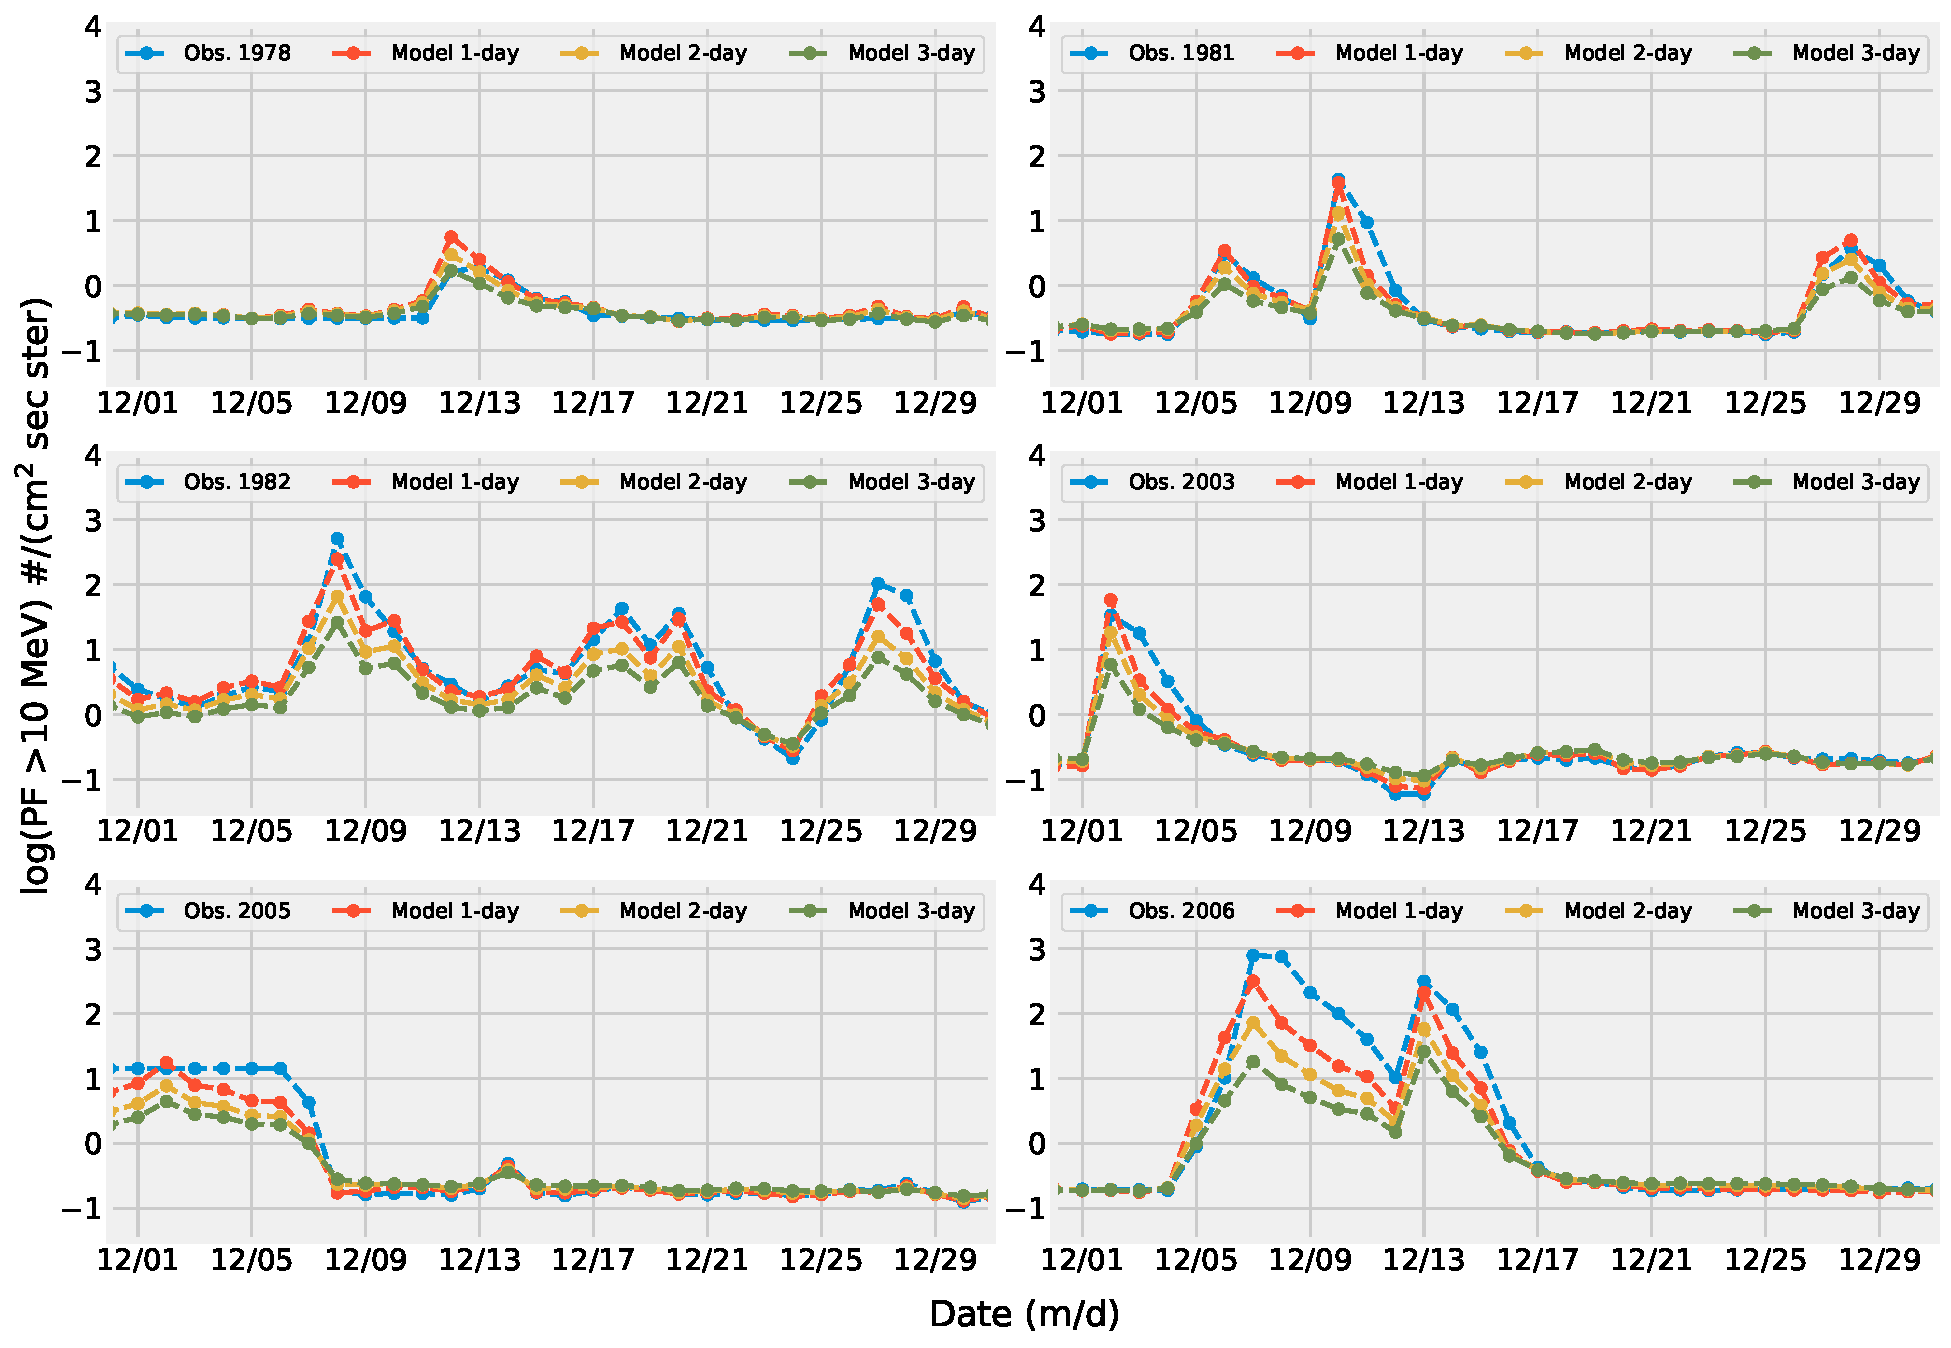
\includegraphics[width=\textwidth]{chapter4/figs/log_pf10/examples_10_tstset.pdf}
    \caption{The model's forecasts for the out-of-sample testing set for the $>$10 MeV channel are shown at forecast horizons of 1 day, 2 days, and 3 days ahead, using samples of data from December in selected years mentioned in the top-left side of the plots.}
\label{fig_examples_pf10_tstset}
\end{figure}

\begin{table}[!htp]
\centering
\caption{Summary of the performance results of the models for the validation and test sets.}
\begin{tabular}{lccccccccl}
\hline
\multicolumn{10}{c}{\textbf{Validation Set}}                                                                                                                 \\ \hline
       & \multicolumn{3}{c}{log PF \textgreater{}10 MeV} & \multicolumn{3}{c}{log PF \textgreater{}30 MeV} & \multicolumn{3}{c}{log PF \textgreater{}60 MeV} \\ \hline
Model Loss   & \multicolumn{3}{c}{0.0016}                      & \multicolumn{3}{c}{0.0010}                      & \multicolumn{3}{c}{0.0009}                      \\
Model Metric & \multicolumn{3}{c}{0.0329}                      & \multicolumn{3}{c}{0.0232}                      & \multicolumn{3}{c}{0.0218}                      \\ \hline
       & 1-Day          & 2-Day          & 3-Day         & 1-Day          & 2-Day          & 3-Day         & 1-Day    & 2-Day   & \multicolumn{1}{c}{3-Day}  \\ \hline
MAE    & 0.061          & 0.091          & 0.125         & 0.053          & 0.079          & 0.098         & 0.052    & 0.069   & 0.086                      \\
MSE    & 0.013          & 0.028          & 0.054         & 0.010          & 0.031          & 0.055         & 0.009    & 0.027   & 0.047                      \\
RMSE   & 0.114          & 0.168          & 0.233         & 0.098          & 0.176          & 0.234         & 0.097    & 0.164   & 0.217                      \\
MAPE   & 22.156         & 28.104         & 34.721        & 13.039         & 18.590         & 22.735        & 10.036   & 13.994  & 16.731                     \\ \hline
\multicolumn{10}{c}{\textbf{Test Set}}                                                                                                                       \\ \hline
       & \multicolumn{3}{c}{log PF \textgreater{}10 MeV} & \multicolumn{3}{c}{log PF \textgreater{}30 MeV} & \multicolumn{3}{c}{log PF \textgreater{}60 MeV} \\ \hline
Model Loss   & \multicolumn{3}{c}{0.0014}                      & \multicolumn{3}{c}{0.0011}                      & \multicolumn{3}{c}{0.0010}                      \\
Model Metric & \multicolumn{3}{c}{0.0333}                      & \multicolumn{3}{c}{0.0283}                      & \multicolumn{3}{c}{0.0250}                      \\ \hline
       & 1-Day          & 2-Day          & 3-Day         & 1-Day          & 2-Day          & 3-Day         & 1-Day    & 2-Day   & \multicolumn{1}{c}{3-Day}  \\ \hline
MAE    & 0.072          & 0.099          & 0.125         & 0.053          & 0.088          & 0.107         & 0.045    & 0.066   & 0.081                      \\
MSE    & 0.015          & 0.030          & 0.050         & 0.009          & 0.029          & 0.048         & 0.007    & 0.020   & 0.034                      \\
RMSE   & 0.121          & 0.172          & 0.224         & 0.094          & 0.170          & 0.218         & 0.082    & 0.141   & 0.184                      \\
MAPE   & 30.135         & 37.498         & 48.139        & 20.599         & 34.300         & 40.803        & 12.358   & 20.504  & 25.305                     \\ \hline
\end{tabular}
\label{table_performance}
\end{table}

\begin{table}[!htp]
\centering
\caption{Confusion matrix for the energy channel $\geq$10 MeV predictions in the test set.}
\label{table_skillscores}
%\begin{tabular}{lccccccccccc}
\begin{tabular}{lccccc}
	\hline
	\bf{E \textgreater{}10 MeV} & \bf{No. events} & \bf{TP} & \bf{TN} & \bf{FP} & \bf{FN} \\ \hline
	1-day ahead            & 15         & 21 & 1441 & 2  & 13 \\ \hline
	2-day ahead            & 13         & 14 & 1441 & 2  & 20 \\ \hline
	3-day ahead            & 5          & 5  & 1443 & 0  & 29 \\ \hline
	\end{tabular}
\end{table}

\begin{table}[htp]
\centering
\caption{Comparing the skill scores with previous models. The dashed entries mean the data is unavailable (\citet{whitman_2022} for more details).}
\label{table_skillscores_comparison}
\resizebox{\textwidth}{!}{%
\begin{tabular}{lccccccccc}
\hline
\multicolumn{1}{c}{\textbf{Model}}       &            & \textbf{POD} & \textbf{FAR} & \textbf{TSS} & \textbf{HSS} & \textbf{POFD} & \textbf{CSI} & \multicolumn{1}{l}{\textbf{Accuracy}} & \multicolumn{1}{l}{\textbf{Precision}} \\ \hline
\multirow{3}{*}{Our BiLSTM model}        & 1-Day      & 0.618        & 0.087        & 0.531        & 0.732        & 0.001         & 0.583        & 0.99                                  & 0.913                                  \\ \cline{2-10} 
                                         & 2-Day      & 0.412        & 0.125        & 0.287        & 0.553        & 0.001         & 0.389        & 0.985                                 & 0.875                                  \\ \cline{2-10} 
                                         & 3-Day      & 0.147        & 0            & 0.147        & 0.252        & 0             & 0.147        & 0.980                                 & 1                                      \\ \hline
\multicolumn{2}{l}{UMASEP-10 \citep{nunez_2011}}           & 0.822        & 0.219        & ---          & ---          & ---           & ---          & ---                                   & ---                                    \\ \hline
\multicolumn{2}{l}{PCA \citep{papaioannou_2018}}     & 0.587        & 0.245        & ---          & 0.65         & ---           & ---          & ---                                   & ---                                    \\ \hline
\multicolumn{2}{l}{SPARX \citep{dalla_2017}}         & 0.5          & 0.57         & ---          & ---          & 0.32          & 0.3          & ---                                   & ---                                    \\ \hline
\multicolumn{2}{l}{SPRINTS \citep{engell_2017}}      & 0.56         & 0.34         & ---          & 0.58         & ---           & ---          & ---                                   & ---                                    \\ \hline
\multicolumn{2}{l}{REleASE \citep{malandraki_2018}} & 0.63         & 0.3          & ---          & ---          & ---           & ---          & ---                                   & ---                                    \\ \hline
\end{tabular}
}
\end{table}

\subsubsection{Short-term Forecasting}
This study aims to enhance the prediction accuracy of SEP integral flux, crucial for mitigating space weather hazards \citep{mnedal_2023a}. Employing a BiLSTM NN model, it utilizes high-resolution hourly-averaged data from four standard integral GOES channels. Key input parameters include the F10.7 index, sunspot number, x-ray flux, solar wind speed, and IP magnetic field strength, sourced from OMNIWeb and GOES databases across two solar cycles. Additional features, like active region locations from NOAA daily reports, are incorporated for improved predictions.

Evaluation involves out-of-sample testing, assessing feature impacts, and benchmarking against existing methods. Data partitioning follows the 9-2-1 strategy over a 23-year period (1996–2018), with 73.99\%, 16.44\%, and 9.57\% allocated to training, validation, and testing sets respectively. Data formatting adopts the MIMO strategy \citep{benson_2020}.

The model forecasts the logarithm of integral proton flux across energy channels, with a focus on $>$10 MeV. Figure~\ref{fig_sample_pf10_hr} compares 1-hour predictions with observations for two sample SEP events.

\begin{figure}[!htp]
	\centering
	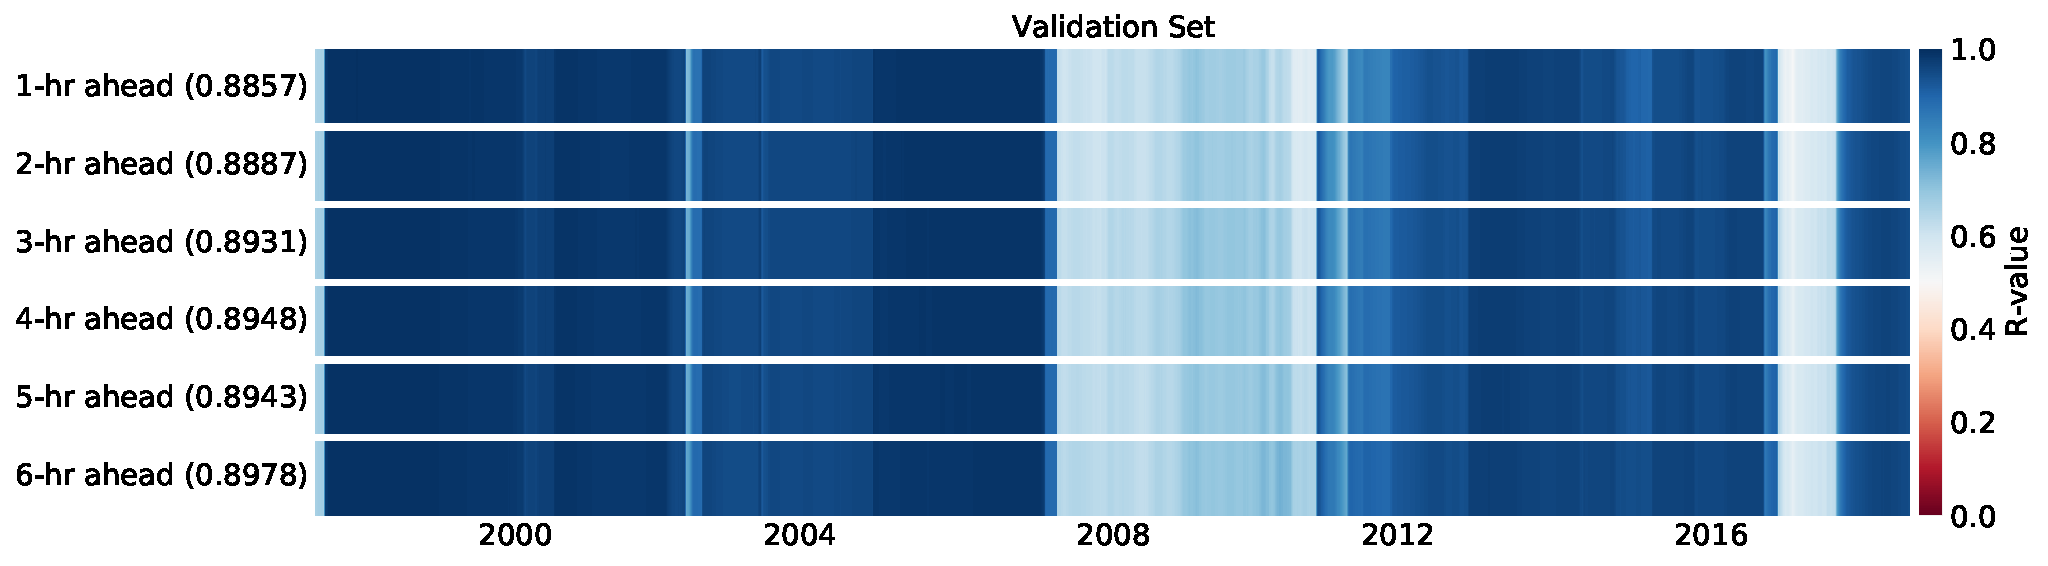
\includegraphics[width=\textwidth]{chapter4/figs/hourly_PF10/temporal_heatmap_val.pdf}
	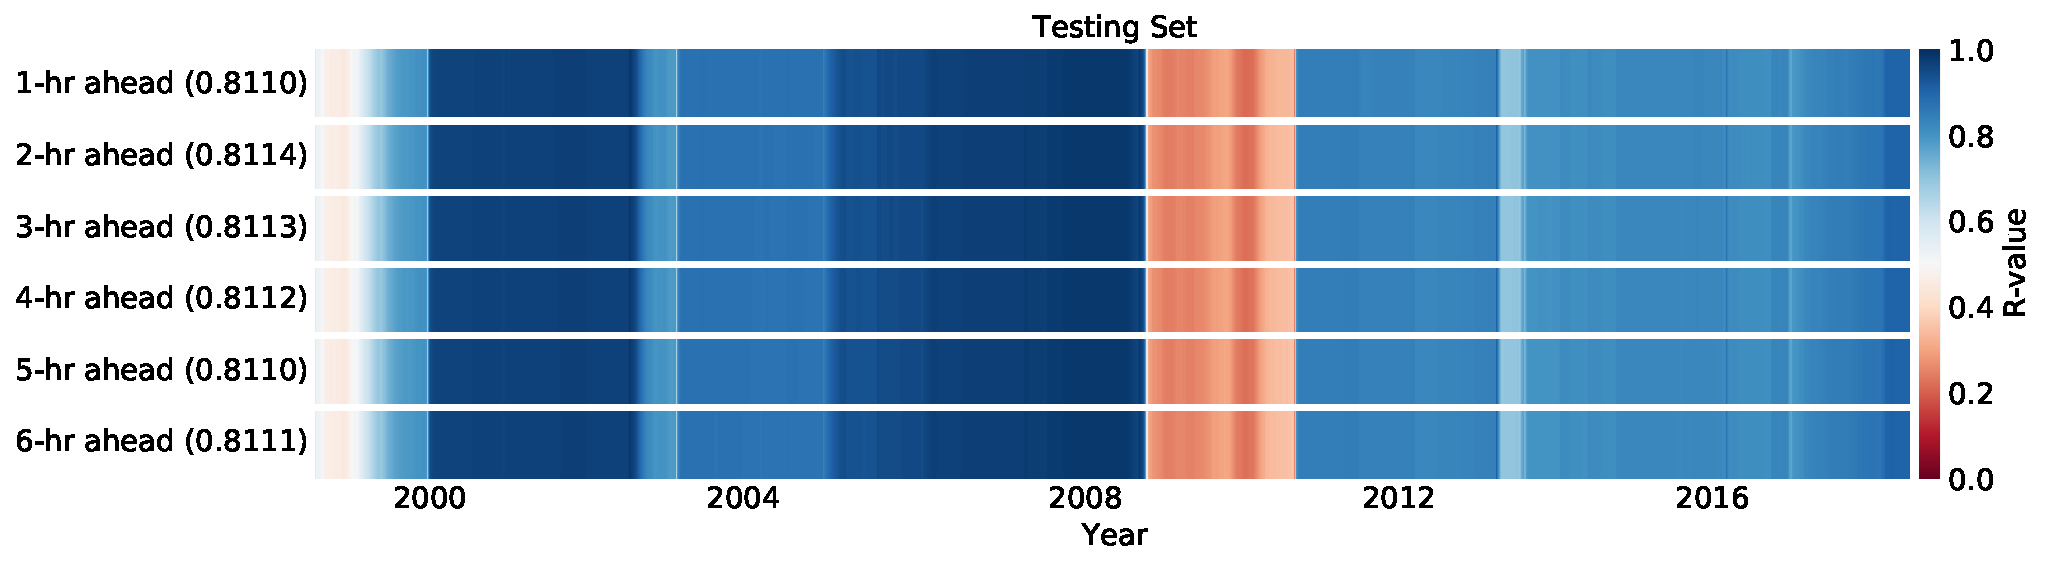
\includegraphics[width=\textwidth]{chapter4/figs/hourly_PF10/temporal_heatmap_test.pdf}
	\caption{Temporal heatmap shows a comparison between the model outputs and observations for the rolling-mean window correlation of the integral $>$10 MeV proton flux at six predicting windows. The top panel represents the validation set and the bottom panel represents the testing set. The numbers on the y-axis are the mean R values.}
	\label{fig_temp_heatmap_valtest}
\end{figure}

\begin{table}[!htp]
	\centering
	\caption{The MSE/MAE for the validation and test sets over six forecasting windows.}
	\label{tab:my-table}
	\resizebox{\columnwidth}{!}{%
		\begin{tabular}{lcccccc}
			\hline
			& 1-hr        & 2-hr        & 3-hr        & 4-hr        & 5-hr        & 6-hr        \\ \hline
			Valid. Set & 0.078/0.238 & 0.086/0.254 & 0.091/0.263 & 0.098/0.273 & 0.102/0.280 & 0.115/0.299 \\ \hline
			Test Set   & 0.012/0.080 & 0.012/0.079 & 0.012/0.080 & 0.011/0.079 & 0.011/0.080 & 0.011/0.079 \\ \hline
		\end{tabular}%
	}
\end{table}

\begin{figure}[!htp]
	\centering
	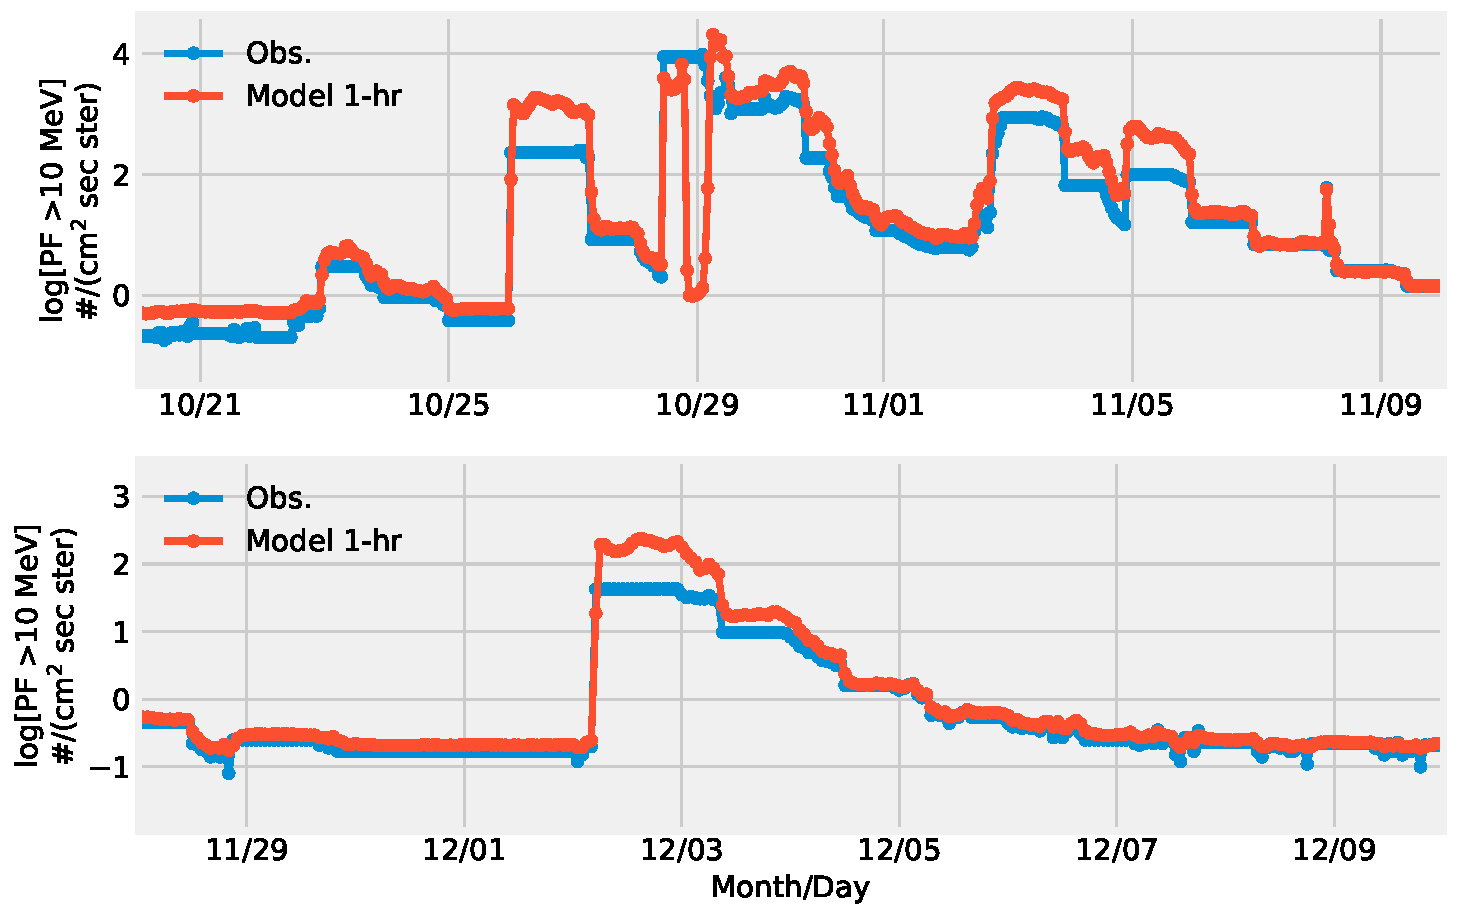
\includegraphics[width=0.7\textwidth]{chapter4/figs/hourly_PF10/sample_valandtestsets_2003.pdf}
	\caption{Comparison between the model’s forecast and the observations for the integral $>$10 MeV proton flux at forecast horizon of 1 hour ahead. The top panel represents a sample of the validation set and the bottom panel represents a sample of the testing set.}
	\label{fig_sample_pf10_hr}
\end{figure}

\section{Conclusions}
In \citet{kozarev_2022}, we pioneer a multi-event exploration, comprehensively examining Sun-to-1 AU SEP simulations utilizing detailed coronal diffusive shock acceleration and interplanetary propagation. Analyzing 62 eruptive events with the SPREAdFAST framework, originally designed for early-stage SEP event forecasting, yielded promising results, showcasing the framework's efficacy.

Input spectra for coronal proton acceleration were derived from quiet-time suprathermal spectra scaled to the Sun. Coronal proton acceleration, influenced by solar corona conditions, exhibited significant impacts on proton acceleration and shock wave surface characteristics.

Comparing DSA model results with SOHO/ERNE instrument observations at 1 AU revealed promising alignment, though discrepancies, particularly at higher energies, were noted. Future work will focus on realistic event modeling, incorporating time-dependent injection of source spectra and three-dimensional transport effects.

In \citet{mnedal_2023a}, BiLSTM neural networks are developed and trained to predict daily-averaged integral flux of SEP at 1-day, 2-day, and 3-day ahead, focusing on energy channels $>$10 MeV, $>$30 MeV, and $>$60 MeV. Input data from OMNIWeb databases span four solar cycles, utilizing MIMO strategy for forecasting, achieving promising results with low MSE values and strong correlations.

The study highlights challenges in longer-term SEP forecasting, particularly in maintaining model performance over extended forecasting windows. Short-term predictions are crucial for space weather forecasting, emphasizing the significance of accurate modeling for protecting space assets.

BiLSTM networks offer promise for heliophysics forecasting tasks, warranting further investigation into optimal model configurations and data requirements. Our study contributes to the growing field of deep learning in heliophysics and space weather research.

In conclusion, our work demonstrates the potential of BiLSTM neural networks in forecasting SEP integral fluxes, essential for space weather forecasting and safeguarding space assets. Future efforts will focus on real-time prediction models, incorporating recent data and enhancing model sophistication for improved accuracy.